\documentclass{article}
\usepackage[margin=0.65in]{geometry}
\usepackage{enumitem}
\usepackage{graphicx}
\usepackage{hyperref}
\usepackage{titlesec}
\usepackage{xcolor}
\hypersetup{hidelinks}
\setlist[itemize]{leftmargin=1.5em,topsep=2pt,itemsep=1pt,parsep=0pt,partopsep=0pt}
\titlespacing*{\section}{0pt}{1.2ex}{0.6ex}
\setlength{\parindent}{0pt}
\setlength{\parskip}{0.5em}
\setlength{\textfloatsep}{8pt}
\setlength{\intextsep}{6pt}
\setlength{\abovecaptionskip}{4pt}
\setlength{\belowcaptionskip}{0pt}
\makeatletter
\renewcommand{\maketitle}{%
    \begin{center}
        {\Large\bfseries \@title\par}\vspace{0.3em}
        {\normalsize \@author\par}\vspace{0.2em}
        {\small \@date\par}
    \end{center}\vspace{0.4em}
}
\makeatother
% HJNotes-Tags: AI Infra, Basics, MPI
% HJNotes-Summary:
\title{Collective Communication in AI Infra}
\author{HJ}
\begin{document}
\maketitle
\section{Collective Communication}
Collective communication is defined as communication that involves a group of processes, these concept used widely in AI Infra:
\begin{itemize}
    \item Broadcast(1:N): 1 member send copies to all group members
    \item Scatter(1:N): 1 member scatter data to all.
    \item Gather(1:N): 1 member gather data from all.
    \item AllGather(N:N): Each member gather data from all, everyone should have the complete and same dataset.
    \item All2All(N:N): Change the datalayout by dispatch+combine, here the example did Matrix Transpose.
\end{itemize}

\begin{figure}[!ht]
    \centering
    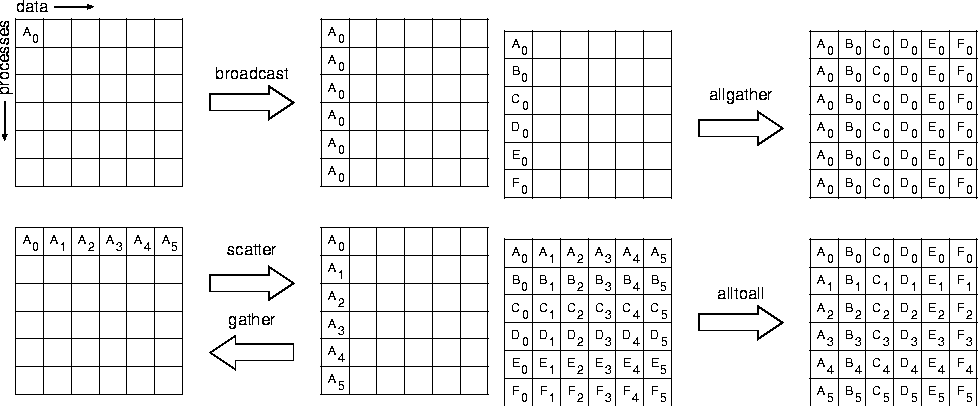
\includegraphics[width=\linewidth,height=0.52\textheight,keepaspectratio]{CollectiveCommunication.png}
    \caption{Collective communication patterns for six processes, from the MPI-1.1 standard~\cite{mpi-collective}.}
\end{figure}

\section{About Reduce}
\textcolor{red}{TODO: Should read slides about ReduceScatter, Allgather in LLM, and AllReduce in MPI}

\begin{thebibliography}{1}
    \bibitem{mpi-collective}
    MPI Forum, \emph{MPI: A Message-Passing Interface Standard}, Version 1.1,
    Section 4.1, \href{https://www.mcs.anl.gov/research/projects/mpi/mpi-standard/mpi-report-1.1/node64.htm}{``Introduction and Overview.''}
\end{thebibliography}

\end{document}

